%% Basierend auf einer TeXnicCenter-Vorlage von Tino Weinkauf.
%%%%%%%%%%%%%%%%%%%%%%%%%%%%%%%%%%%%%%%%%%%%%%%%%%%%%%%%%%%%%%

%%%%%%%%%%%%%%%%%%%%%%%%%%%%%%%%%%%%%%%%%%%%%%%%%%%%%%%%%%%%%
%% HEADER
%%%%%%%%%%%%%%%%%%%%%%%%%%%%%%%%%%%%%%%%%%%%%%%%%%%%%%%%%%%%%
\documentclass[a4paper,twoside,12pt]{article}
% Alternative Optionen:
%	Papiergr��e: a4paper / a5paper / b5paper / letterpaper / legalpaper / executivepaper
% Duplex: oneside / twoside
% Grundlegende Fontgr��en: 10pt / 11pt / 12pt

%% Deutsche Anpassungen %%%%%%%%%%%%%%%%%%%%%%%%%%%%%%%%%%%%%
\usepackage[ngerman]{babel}
\usepackage[T1]{fontenc}
\usepackage[ansinew]{inputenc}
\usepackage{setspace}
\usepackage{cancel} % strikethrough in math mode
\usepackage[osf]{mathpazo}	% Mathpazo package includes accompanying math fonts

\usepackage{lmodern} %Type1-Schriftart f�r nicht-englische Texte

%% Packages f�r Grafiken & Abbildungen %%%%%%%%%%%%%%%%%%%%%%
\usepackage{graphicx} %%Zum Laden von Grafiken
\usepackage{graphics}
%\usepackage{subfig} %%Teilabbildungen in einer Abbildung
%\usepackage{tikz} %%Vektorgrafiken aus LaTeX heraus erstellen
%\usepackage{qtree}

%% Packages f�r Formeln %%%%%%%%%%%%%%%%%%%%%%%%%%%%%%%%%%%%%
\usepackage{amsmath}
\usepackage{amsthm}
\usepackage{amsfonts}

%% Zeilenabstand %%%%%%%%%%%%%%%%%%%%%%%%%%%%%%%%%%%%%%%%%%%%
\usepackage{setspace}
\singlespacing        %% 1-zeilig (Standard)

%% Andere Packages %%%%%%%%%%%%%%%%%%%%%%%%%%%%%%%%%%%%%%%%%%
\usepackage{a4wide} %%Kleinere Seitenr�nder = mehr Text pro Zeile.
\usepackage{fancyhdr} %%Fancy Kopf- und Fu�zeilen
%\renewcommand{\headheight}{15pt}
\usepackage{fancybox}

%\usepackage{longtable} %%F�r Tabellen, die eine Seite �berschreiten
%\usepackage{ifpdf}
%\ifpdf
	\usepackage[hyperindex,colorlinks,bookmarks,urlcolor=blue]{hyperref}
%\else
%	\usepackage{url}
%\fi

%% FancyHeader Definitionen %%%%%%%%%%%%%%%%a%%%%%%%%%%%%%%%%%%%%%%%%%%

%\lhead{Stchastik A, WS 2009}
%\chead{}
%\rhead{Mitschrift}

%\pagestyle{fancy}{
%	\fancyhead[LO,RE]{\rightmark}
%	\fancyhead[RO,LE]{\leftmark}
%	\fancyfoot[C]{\thepage}
%}

%\renewcommand{\sectionmark}[1]{\markright{#1}}
%\renewcommand{\subsectionmark}[1]{\markleft{#1}}

%% Basierend auf einer TeXnicCenter-Vorlage von Tino Weinkauf.

%%%%%%%%%%%%%%%%%%%%%%%%%%%%%%%%%%%%%%%%%%%%%%%%%%%%%%%%%%%%%%


%%%%%%%%%%%%%%%%%%%%%%%%%%%%%%%%%%%%%%%%%%%%%%%%%%%%%%%%%%%%%

%% OPTIONEN

%%%%%%%%%%%%%%%%%%%%%%%%%%%%%%%%%%%%%%%%%%%%%%%%%%%%%%%%%%%%%

%%

%% ACHTUNG: Sie ben�tigen ein Hauptdokument, um diese Datei

%%          benutzen zu k�nnen. Verwenden Sie im Hauptdokument

%%          den Befehl "\input{dateiname}", um diese

%%          Datei einzubinden.

%%



%%%%%%%%%%%%%%%%%%%%%%%%%%%%%%%%%%%%%%%%%%%%%%%%%%%%%%%%%%%%%

%% ABK�RZUNGEN

%%%%%%%%%%%%%%%%%%%%%%%%%%%%%%%%%%%%%%%%%%%%%%%%%%%%%%%%%%%%%


%%Definitionen f�r Abbildung-Referenzen

\newcommand{\abb}[1]{(Abbildung \ref{#1})}

\newcommand{\ABB}[1]{Abbildung \ref{#1}}


%%Definitionen f�r Tabellen-Referenzen

\newcommand{\tab}[1]{(Tabelle \ref{#1})}

\newcommand{\TAB}[1]{Tabelle \ref{#1}}


%%Definitionen f�r Seiten-Referenzen

\newcommand{\seite}[1]{(Seite \pageref{#1})}

\newcommand{\SEITE}[1]{Seite \pageref{#1}}


%%Definitionen f�r Code

\newcommand{\precode}[1]{\textbf{\footnotesize #1}}

\newcommand{\code}[1]{\texttt{\footnotesize #1}}


%% Basierend auf einer TeXnicCenter-Vorlage von Tino Weinkauf.

%%%%%%%%%%%%%%%%%%%%%%%%%%%%%%%%%%%%%%%%%%%%%%%%%%%%%%%%%%%%%%


%%%%%%%%%%%%%%%%%%%%%%%%%%%%%%%%%%%%%%%%%%%%%%%%%%%%%%%%%%%%%

%% OPTIONEN

%%%%%%%%%%%%%%%%%%%%%%%%%%%%%%%%%%%%%%%%%%%%%%%%%%%%%%%%%%%%%

%%

%% ACHTUNG: Sie ben�tigen ein Hauptdokument, um diese Datei

%%          benutzen zu k�nnen. Verwenden Sie im Hauptdokument

%%          den Befehl "\input{dateiname}", um diese

%%          Datei einzubinden.

%%


%%%%%%%%%%%%%%%%%%%%%%%%%%%%%%%%%%%%%%%%%%%%%%%%%%%%%%%%%%%%%

%% OPTIONEN F�R ABST�NDE

%%%%%%%%%%%%%%%%%%%%%%%%%%%%%%%%%%%%%%%%%%%%%%%%%%%%%%%%%%%%%


%%Abstand zwischen den Abs�tzen: halbe H�he vom kleinen x

\setlength{\parskip}{0.5ex}


%%Einzug am Anfang eines Absatzes: auf Null setzen

%\setlength{\parindent}{0ex}


%%Zeilenabstand: 1.5 fach

%% ==> Erw�gen Sie, anstelle dieses Kommandos das Paket 'setspace' zu verwenden.

%\linespread{1.5}



%%%%%%%%%%%%%%%%%%%%%%%%%%%%%%%%%%%%%%%%%%%%%%%%%%%%%%%%%%%%%

%% OPTIONEN F�R KOPF- UND FUSSZEILEN

%%%%%%%%%%%%%%%%%%%%%%%%%%%%%%%%%%%%%%%%%%%%%%%%%%%%%%%%%%%%%

%%Beispiel f�r recht nette Kopf- und Fu�zeilen

%% ==> Nutzen Sie '\usepackage{fancyhdr}' und '\pagestyle{fancy}'

%% ==> im Hauptdokument, um diese zu benutzen.

%\pagestyle{fancy}

\renewcommand{\chaptermark}[1]{\markboth{#1}{}}

\renewcommand{\sectionmark}[1]{\markright{\thesection\ #1}}

\fancyhf{}

\fancyhead[LE,RO]{\thepage}

\fancyhead[LO]{\rightmark}

\fancyhead[RE]{\leftmark}

\fancypagestyle{plain}{%

    \fancyhead{}

    \renewcommand{\headrulewidth}{0pt}

}



%% Basierend auf einer TeXnicCenter-Vorlage von Tino Weinkauf.

%%%%%%%%%%%%%%%%%%%%%%%%%%%%%%%%%%%%%%%%%%%%%%%%%%%%%%%%%%%%%%


%%%%%%%%%%%%%%%%%%%%%%%%%%%%%%%%%%%%%%%%%%%%%%%%%%%%%%%%%%%%%

%% PDF-Informationen

%%%%%%%%%%%%%%%%%%%%%%%%%%%%%%%%%%%%%%%%%%%%%%%%%%%%%%%%%%%%%

%%

%% ACHTUNG: Sie ben�tigen ein Hauptdokument, um diese Datei

%%          benutzen zu k�nnen. Verwenden Sie im Hauptdokument

%%          den Befehl "\input{dateiname}", um diese

%%          Datei einzubinden.

%%


\pdfinfo{                               % Zusatzinformationen in PDF-Datei;

                                        % alle Werte sind optional.

    /Author (Ronald Becher)

    /CreationDate (D:20090928120000)    % Datum der Erstellung

                                        % (D:JJJJMMTThhmmss)

                                        % JJJJ  Jahr

                                        % MM    Monat

                                        % TT    Tag

                                        % hh    Stunden

                                        % mm    Minuten

                                        % ss    Sekunden

                                        %

                                        % Standard: Das aktuelle Datum

                                        %

    /ModDate (\date)         % Datum der letzten Modifikation

    /Creator (TeX && TXC)               % Standard: "TeX"

    /Producer (pdfTeX)                  % Standard: "pdfTeX" + pdftex version

    /Title (Vorlesungsmitschrift Stochastik Wintersemester 2009)

    /Subject (Thema Ihres Dokumentes)

    /Keywords (stochastik, mathematik, vorlesung, mitschrift)

}




\title{Stochastik Wintersemester 2009\\Leibniz Universit�t Hannover\\Vorlesungsmitschrift}

\author{Dozent: \href{mailto:lbaring@stochastik.uni-hannover.de}{Prof. Dr. L. Baringhaus}\\ \vspace{1em} \\
Mitschrift von\\
\href{mailto:rb@ronald-becher.com}{Ronald Becher}}

\begin{document}
\pagestyle{empty}
\maketitle
\begin{abstract}
	Diese Mitschrift wird erstellt im Zuge der Vorlesung \href{http://www.stochastik.uni-hannover.de/bachws09/index.html}{Stochastik A} im Wintersemester 2009 an der \href{http://www.uni-hannover.de}{Leibniz Universit�t Hannover}. Obwohl mit gro\ss er Sorgfalt geschrieben, werden sich sicherlich Fehler einschleichen. Diese bitte ich zu melden, damit sie korrigiert werden k�nnen. Ihr k�nnt euch dazu an jeden der genannten Autoren (mit Ausnahme des Dozenten) wenden.
	
	Dieses Skript wird prim�r �ber \href{http://github.com/rbecher/luh-vorlesungen-inf-ws09-stoch}{Github} verteilt und "`gepflegt"'. Dort kann man es auch forken, verbessern und dann (idealerweise) ein "`Pull Request"' losschicken. Siehe auch  \href{http://github.com/guides}{Github Guides}. Auch wenn ihr gute Grafiken zur Verdeutlichung beitragen k�nnt, d�rft ihr diese gerne schicken oder selbst einf�gen (am besten als \LaTeX -geeignete Datei (Tikz, SVG, PNG, \dots)).
	
	\textbf{Hinweis}: Es wird o.B.d.A. davon abgeraten, die Vorlesung zu vers�umen, nur weil eine Mitschrift angefertigt wird! Selbiges gilt f�r den �bungsbetrieb! Stochastik besteht ihr nur, wenn ihr auch zu der Veranstaltung geht!
\end{abstract}

\newpage % \newpage works far better than \pagebreak

\tableofcontents

%Part: F�r gro�e Themenbl�cke (z.B. Einf�hrung, Kombinatorik, etc)
%Section: F�r Abschnitte (z.B. Mengen, von Mengen zu anderen Mengen, etc)
%Subsection: Beweise, S�tze, Lemmata

\newpage

\pagestyle{fancy}
\addtolength{\headheight}{\baselineskip}
\renewcommand{\sectionmark}[1]{\markboth{#1}{}}
\renewcommand{\subsectionmark}[1]{\markright{#1}}
%\rhead{\leftmark\\\rightmark}
\fancyhead[LE,RO]{Mitschrift Stochastik A, WS 2009}
\fancyhead[LO,RE]{\leftmark\\\rightmark}
% Here comes content

\part{Einf�hrung / Organisatorisches}
\label{sec:Einf�hrungOrganisatorisches}

\par Die Klausur wird am \textbf{01.02.2010 von 9:15 - 10:45} stattfinden, es wird w�chentliche Haus- und Stunden�bungen geben.\\
Die abgegebenen Haus�bungen werden korrigiert und in den �bungsgruppen zur�ckgegeben werden, es gibt allerdings keine Bonuspunkteregelung.
�bungsgruppen wird es folgende geben:
\begin{itemize}
	\item Mo, 12:15 - 13:00 Uhr (F309)
	\item Mo, 14:15 - 15:00 Uhr (G123) [max. 20 Teilnehmer]
	\item Di, 10:15 - 11:00 Uhr (F428)
	\item Di, 12:15 - 13:00 (F442)
	\item Mi, 12:15 - 13:00 (B305)
\end{itemize}

\newpage

\part{Wahrscheinlichkeitstheorie}
\label{sec:Wahrscheinlichkeitstheorie}

"`Was ist das richtige Modell, um ein Experiment zu beschreiben?"' ist die wichtigste Frage, die die mathematische Statistik zu beantworten hat, und diese Modelle an die Wirklichkeit anzupassen, ist die haupts�chliche Aufgabe der Stochastik. Der letzte Teil wird vor allem in der Vorlesung \textbf{Stochastik B} behandelt.

\section{Wahrscheinlichkeitsr�ume}
\label{sec:Wahrscheinlichkeitsr�ume}

Zufallsexperimente werden beschrieben durch
\begin{itemize}
	\item die Menge der m�glichen Ergebnisse $\Omega$\\
	Im \textbf{W�rfelwurf} sei beispielsweise $\Omega := \{1,2,3,4,5,6\}$
	\item die Menge $\mathfrak{A}$ $\subset \mathfrak{P}(\Omega):=\{A; A\subset\Omega\}$ als Menge der interessierenden Ergebnisse.\\
	$\mathfrak{A}$ ist eine so genannte \href{http://de.wikipedia.org/wiki/Sigma-Algebra}{$\sigma$-Algebra} auf $\Omega$, d.h. 
	\begin{enumerate}
	\item $\Omega \in \mathfrak{A}$.\\(Die Grundmenge $\Omega$ ist in $\mathfrak{A}$ enthalten)
	\item Mit $A \in \mathfrak{A} \Leftrightarrow A^c \in \mathfrak{A}$.\\ (Wenn $\mathfrak{A}$ eine Teilmenge $A\in\Omega$ als m�gliches Ergebnis enth�lt, dann auch deren Komplement $A^c=\Omega \setminus A$)
	\item Mit $A_1,A_2,\dots\in \mathfrak{A}$ ist auch $\bigcup_{n=1}^{\infty}A_n\in \mathfrak{A}$.\\
	(Wenn f�r jede nat�rliche Zahl $n$ die Menge $A_n \in \mathfrak{A}$ ist, so ist auch die abz�hlbare Vereinigung aller $A_n\in\mathfrak{A}$)
\end{enumerate}
	Im \textbf{W�rfelwurf} seien beispielsweise g�ltige Ereignisse:
	\begin{itemize}
	\item $A := \{2,4,6\}$ das Ergeignis "`Es f�llt eine gerade Zahl"', und
	\item $A := \{5,6\}$ das Ergeignis "`Es f�llt eine Zahl gr�\ss er gleich 5"'.
\end{itemize}
	\item durch ein \href{http://de.wikipedia.org/wiki/Wahrscheinlichkeitsmass}{Wahrscheinlichkeitsma\ss}\ $P$ (lat: "`\textbf{P}robabilitas"'=Glaubw�rdigkeit) mit \linebreak[4] $P:\mathfrak{A} \rightarrow [0,1]$, also eine Mengenfunktion auf $\mathfrak{A}$ mit den Eigenschaften
	\begin{enumerate}
	\item \begin{equation}
		P(\Omega)=1
	\end{equation}
	\textit{(Die so genannte ``Normiertheit'').}
	\item F�r jede Folge von \textbf{paarweise disjunkten} $A_1,A_2,\dots\in \mathfrak{A}$ gilt:
	\begin{equation}
		P\left(\bigcup_{n=1}^{\infty}A_n\right)=\sum_{n=1}^{\infty}{P(A_n)}
	\end{equation}
	\[\sigma\text{-Additivit�t von }P\]
	\noindent F�r $A\in \mathfrak{A}$ ist $P(A)$ die Wahrscheinlichkeitsfunktion (f�r das Eintreten) von A
\end{enumerate}
\end{itemize}

\par\noindent Das Tripel $(\Omega,\mathfrak{A},P)$ hei\ss t \href{http://de.wikipedia.org/wiki/Wahrscheinlichkeitsraum}{\textbf{Wahrscheinlichkeitsraum}}.\\

\par\noindent $\omega\in\Omega$ nennen wir das Ergebnis des Zufallsexperimentes. Das Ereignis $A\in \mathfrak{A}$ tritt genau dann ein, wenn $\omega\in A$.
\begin{equation}
\label{ }
\omega\in\bigcup_{n=1}^{\infty}A_n \iff \exists n\in \mathbb{N} \wedge \omega\in A_n
\end{equation}
Das durch $\bigcup_{n=1}^{\infty}A_n$ beschriebene Ereignis tritt genau dann ein, wenn mindestens eines der Ereignisse $A_n,\ n\in \mathbb{N}$ eintritt.

\noindent Auf die Frage, ob auch $\emptyset$ eine g�ltige Menge ist, sei gesagt, dass \[\emptyset =\Omega^c \in \mathfrak{A}\] das "`unm�gliche Ereignis"' genannt wird (Die Antwort ist also ``ja'').\\

\noindent Seien $A_1,A_2,\ldots \in \mathfrak{A}$. Dann 
\begin{equation}
\bigcap_{n=1}^{\infty}{A_n}=\left(\bigcup_{n=1}^{\infty}A_n^c\right)^c\in \mathfrak{A}
\end{equation}
Anmerkung: $\bigcap_{n=1}^{\infty}A_n$ tritt genau dann ein, wenn alle $A_n,n\in \mathbb{N}$ eintreten.\\

\par\noindent Wenn nun $A,B \in \mathfrak{A}$, dann gilt
\begin{itemize}
	\item \[A\cup B = A\cup B \cup \emptyset \cup \emptyset \cup \dots \in \mathfrak{A}\]
	(Die Vereinigung von $A,B$ ist auch ein interessierendes Ereignis und steht f\"ur ``das Ereignis $A$ oder $B$ treten ein'')
	\item \[A\cap B = A\cap B \cap \Omega \cap \Omega \cap \dots \in \mathfrak{A}\]
	(Die Schnittmenge von $A,B$ ist auch ein interessierendes Ereignis und steht f\"ur ``das Ereignis $A$ \textbf{und} $B$ treten ein'')
	\item \[A \Delta B = (A\cap B^c) \cup (B\cap A^c)\]
	(Die ``symmetrische Differenz'' beschreibt das Ereignis ``Entweder A oder B'')
	\item $A \subseteq B$ hei{\ss}t: ``Das Ereignis A hat das Ereignis B zur Folge''.\\
	(Kurz erkl\"art: Wenn $A$ eintritt, folgt $\omega \in A\ \wedge\ A \subseteq B \Rightarrow \omega \in B$)
\end{itemize}

\subsection{Eigenschaften von Wahrscheinlichkeits-Ma{\ss}en}

\begin{itemize}
	\item Aus $P(\emptyset)=P(\emptyset\cup\emptyset\cup\dots)=\sum_{n=1}^{\infty}{P(\emptyset)}$ folgt $P(\emptyset)=0$.
	\item F�r $A,B\in \mathfrak{A}$ mit $A\subseteq B$ ist 
	\begin{equation}
P(B)=P(A \cup B \cap A^c)=P(A \cup B \cap A^c \cup \emptyset \cup \dots)=P(A)+P(B \cap A^c) \geq P(A)
\end{equation}
	Also gelten folgende Eigenschaften / Gesetzm\"a{\ss}igkeiten
	\begin{itemize}
	\item $P(A)\leq P(B)$ (Isotonie)
	\item $P(B \cap A^c)=P(B)-P(A)$ (Subtraktivit�t)
\end{itemize}
\end{itemize}

\subsection{Beispiel}

$\emptyset \neq \Omega$ sei endlich, $|\Omega|$ Anzahl der Elemente von $\Omega$ und $\mathfrak{A}=\mathfrak{P}(\Omega)$.\\
Sei $P$ definiert durch 
\begin{equation}
P(A)=\frac{|A|}{|\Omega|},\ A \subset \Omega
\end{equation}
$P$ hei\ss t "`diskretes Laplace'sches W-Ma\ss "` auf $\Omega$.\\
Es ist 
\begin{equation}
P(\{\omega\})=\frac{1}{|\Omega|},\ \omega\in\Omega
\end{equation}
also folgert man: "`Alle m�glichen Ergebnisse sind \textbf{gleich wahrscheinlich}."'

\newpage

\section{Grundformeln der Kombinatorik}
\label{sec:Grundformeln der Kombinatorik}

$n,r\in \mathbb{N}$, $M_n$ ist eine $n$-elementige Menge, o.B.d.A. $M_n=\{1,\ldots,n\}$.
\begin{itemize}
	\item 
	\begin{equation}
P_n^{r}=\{(x_1,\dots,x_r);\ x_i \in M_n, 1 \leq i \leq r\}
\end{equation}
	das sind die $r$-\href{http://de.wikipedia.org/wiki/Permutation}{Permutationen} aus $M_n$ mit Wiederholung.
	\item 
	\begin{equation}
	P_n^{(r)}=\{(x_1,\dots,x_r);\ x_i \in M_n, 1 \leq i \leq r, \text{paarweise\ verschieden}\}\ (r \leq n)
\end{equation}
	das sind die $r$-Permutationen aus $M_n$ ohne Wiederholung.
	\item 
	\begin{equation}K_n^{(r)}=\{(x_1,\dots,x_r);\ x_i \in M_n, 1 \leq i \leq r,\ x_1 < x_2 < \dots < x_n\}\ (r \leq n)
\end{equation}
	das sind die $r$-Kombinationen aus $M_n$ ohne Wiederholung.
	\item 
	\begin{equation}K_n^{r}=\{(x_1,\dots,x_r);\ x_i \in M_n, 1 \leq i \leq r,\ x_1 \leq x_2 \leq \dots \leq x_n\}\ (r \leq n)
\end{equation}
	das sind die $r$-Kombinationen aus $M_n$ mit Wiederholung.
\end{itemize}

\subsection{Zur Erkl\"arung}
\begin{enumerate}
	\item Tupel in Permutationen sind nicht angeordnet, hier ist die Reihenfolge wichtig!
  \item Tupel in Kombinationen sind o.B.d.A. angeordnet, wir k\"onnen sie also ``vergleichen''.
  \item Bei Varianten \textbf{mit Wiederholung}, d\"urfen also zwei Elemente ``nebeneinander'' auch gleich sein, bei Varianten \textbf{ohne Wiederholung} ist das nicht der Fall, hier m\"ussen die Elemente also echt unterschiedlich sein.
  \item Bei einer $r$-Permutation/Kombination haben wir eine $r$-elementige Teilmenge (die also kleiner oder gleich gro{\ss} der ``gro{\ss}en'' Menge $M_n$ ist).
  \item ``mit Wiederholung'' nennt man auch ``mit Zur\"ucklegen''
\end{enumerate}

\subsection{Anschauliche Beispiele}
\begin{itemize}
	\item Bei Kombinationen interessiert uns ausschlie�lich, welche Elemente wir aus $M_n$ bekommen, ein gutes Beispiel f�r eine Kombination
	\begin{description}
	\item[ohne Wiederholung] ist also das �bliche Lotto-Spiel ``6 aus 49''. Hier ist es uns egal, ob die Reihenfolge $(1,2,3,4,5,6)$ ist oder $(6,5,4,3,2,1)$.
	\item[mit Wiederholung] ist die Frage, ob wir mindestens zwei Mal in f�nf Versuchen eine Zahl $\geq 5$ w�rfeln
\end{description}
	\item Bei Permutationen interessiert uns neben der Auswahl auch die Anordnung (man sagt: die Elemente sind ``unterscheidbar''). Eine Permutation
	\begin{description}
	\item[ohne Wiederholung] ist z.B. ein Kinobesuch. Ob Tim zwischen Tina und Claudia sitzt, ist f�r ihn nicht gleichwertig mit der Variante, zwischen Klaus und J�rgen zu sitzen.
	\item[mit Wiederholung] ist die Frage, ob ich beim Roulette einen aufsteigenden Run habe, also erst eine $0$ f�llt, dann eine $1$, dann eine $2$, usw. Das Standardbeispiel hierbei ist eine Urne, wo ich Kugeln oder Zettel heraushole und wieder hereinlege.
\end{description}
\end{itemize}

\subsection{Rechnen mit Permutationen und Kombinationen}
Es gilt
\begin{itemize}
	\item 
	\begin{equation}
		|P_n^r|=n^r
	\end{equation}
	\textit{(Erkl�rung: Man greift $r$ Mal in die Urne, schaut sich einen der $n$ Zettel an und legt ihn wieder herein, es gibt also danach genauso viele M�glichkeiten zu ziehen (also $n$))}
	\item
	\begin{equation}
		|P_n^{(r)}|=
		\begin{cases}
		r\leq n\ 	& n\cdot(n-1)\cdot\ldots\cdot(n-r+1) \\[0.5em]
		r=n\ 			& r!
		\end{cases}
	\end{equation}
	\textit{(Erkl�rung: Lege ich meine Zettel nicht wieder in die Urne zur�ck, habe ich beim n�chsten Versuch nat�rlich eine M�glichkeit weniger, welche Zettel ich ziehen k�nnte)}
	\item 
	\begin{align}
		r!\cdot|K_n^{(r)}|	&=|P_n^{(r)}| \label{lab2.3.1}\\
												& \Updownarrow \nonumber \\
		|K_n^{(r)}|					&=\frac{n(n-1)\dots(n-r+1)}{r!}	&=\binom{n}{r} \label{lab2.3.2}\\
												& \Downarrow \nonumber \\
		&|\{A; A\subset M_n, |A|=r\}|^r&=\binom{n}{r} \label{lab2.3.3} \\
												& \Downarrow \nonumber \\
		|\mathfrak{P}(M_n)|	&=\sum_{r=0}^{r}{\binom{n}{r}1^r1^{n-r}}=(1+1)^n &=2^n \label{lab2.3.4}
	\end{align}
	\eqref{lab2.3.3} Gilt auch noch f�r $r=0$.\\
	\textit{(Erkl�rung: \eqref{lab2.3.1} und �quivalent \eqref{lab2.3.2} kann man sich so vorstellen, dass man sich seine $r$-elementige Teilmenge (ohne Zur�cklegen) zusammensuchen kann, aber die verschiedenen M�glichkeiten, sie zu permutieren (``die Kinobesucher umzusetzen''), interessieren den Betrachter hier nicht, also m�ssen wir die aus der Rechnung rausnehmen.)}
	\item $K_n^r \rightarrow (x_1,\dots,x_r) \underbrace{\longrightarrow}_{ist\ bijektiv} (x_1,x_1+1,\dots,x_r+r-1)\in K_{n+r-1}^{(r)}$\\
	$\Rightarrow |K_n^r| = |K_{n+r-1}^{(r)}| = \stackrel{n+r-1}{r}$\\
	Identifiziere $(x_1,\dots,x_r) \in K_n^r$ mit dem Besetzungszahlvektor $(k_1,\dots,k_n)$,
	wobei $k_i=|\{j\in \{ 1,\dots,r \}; x_j=i\}|,\ 1 \leq i \leq n$. Dann ist $K-1+\dots+k_n=r$.\\
	Dann ist $|\{(K_1,\dots,k_n)\in \mathbb{N}_0^n; k_1+\dots+k_n=r\}|=\binom{n+r-1}{r}$\\
	Folgerung: $|\{(K_1,\dots,k_n)\in \mathbb{N}^n; k_1+\dots+k_n=r\}|=\binom{n+(r-n)-1}{r-n}=\binom{r-1}{r-n}=\binom{r-1}{n-1}, r \geq n$\\
\end{itemize}

\par\noindent Aus der Menge der Permutationen betrachten wir eine spezifische Teilmenge.\\
Sei $k_1,\ldots,k_n \in \mathbb{N}_0$ mit $k_1+\ldots+k_n=r$. Einen so genannter ``Besetzungszahlvektor'' dr�ckt man beispielsweise so aus:
\begin{equation}
	\begin{split}
	& \{(x_1,\ldots,x_n)\in\mathbb{P}_n^r;\ |\{j; j\in\{1,\ldots,r\}, x_j=i\}|=k_i, 1\leq i\leq n\}|\\
	=	& \{(x_1,\ldots,x_n)\in\mathbb{P}_n^r;\ \text{Genau $k_i$ der $r$ Komponenten $(x_1,\ldots,x_r)$ sind gleich $i$}, 1\leq i \leq n\}
	\end{split}
	\label{def:besetzungszahlvektor}
\end{equation}

Die L�nge oder M�chtigkeit dieser Menge ist wie folgt:
\begin{equation*}
	\begin{split}
	 |\ref{def:besetzungszahlvektor}| & = \binom{r}{k_1}\binom{r-k_1}{k_2}\binom{r-k_1-k_2}{k_3}\cdots\binom{r-k1-\ldots-k_{n-1}}{k_n}\\
	 & =	\frac{r!}{k_1!\cancel{(r-k_1)!}}\cdot \frac{\cancel{(r-k_1)!}}{k_2!\cancel{(r-k_1-k_2)!}}\cdots \frac{\cancel{(r-k_1-\ldots-k_n)!}}{k_n!}\\
	 & = \frac{r!}{k_1!\cdots k_n!} % (r-k_1)! durchstreichen ... strike?
	\end{split}
\end{equation*}

% Binomischer Lehrsatz
% => Multinomialer Lehrsatz durch Verallgemeinerung

\subsection{Binomischer Lehrsatz}

Es folgt aus dem (bekannten) binomischen Lersatz durch Verallgemeinerung der multinomiale Lehrsatz.

\begin{equation}
n^r = \sum_{\substack{(k_1,\ldots,k_n)\in\mathbb{N}_0^n\\k_1+\ldots+k_n=r}}{\frac{r!}{k_1!\cdots k_n!}} % Anzahl der Summanden = n+r-1 �ber r
\label{def:nhochr}
\end{equation}

\begin{equation}
	\begin{split}
	|\ref{def:nhochr}| &= \binom{n+r-1}{r}
	\end{split}
\end{equation}

\subsection{Beispiel}
O.B.d.A. sind $r$ Personen im Raum, $n=365$ seien die Anzahle der Tage im Jahr und $r\leq n$.\\
Gesucht: Wahrscheinlickeit, dass mindestens $2$ der $r$ Personen am gleichen Tag Geburtstag haben.
\begin{itemize}
	\item $ \Omega = \{ (x_1,\ldots,x_r); x_i \  \} $
	\item $ \mathfrak{A}=\mathfrak{P}(\Omega) $
	\item $ P(A)=\frac{|A|}{|\Omega|}, A\subseteq\Omega $
	\item Alle m�glichen r-Tupel von Geburtstagen sind gleich wahrscheinlich, also
	\item $A= \{ (x_1,\ldots,x_r)\in\Omega; i,j \in \{1,\ldots,r\}, i\neq j, x_i=x_j \}$
	\item $P(A) = 1-P(A^c)$\\
				In vielen F�llen ist es ein valider ``Trick'', statt der Ergebnismenge das Gegenergebnis zu berechnen
	\item $A^c = \{ (x_1,\ldots,x_r)\in\Omega; x_1,\ldots,x_r \text{paarweise verschieden} \}$
	\item $|A^c|=n(n-1)\cdots(n-r+1)$
	\item $P(A)=1- \frac{n(n-1)\cdots(n-r+1)}{n^r}$
\end{itemize}

\begin{equation*}
P(A)=\begin{cases}
> 1/2& \text{wenn $r>23$},\\
0,706& \text{wenn $r=30$},\\
0,994& \text{wenn $r=60$}.
\end{cases}
\end{equation*}

\subsection{Die Siebformel}
	 
Seien $A_1,A_n$ Ereignisse in W-Raum $(\Omega,\mathfrak{A},P)$
\begin{equation}
\begin{split}
P(A_1\cup A_2) 	&= P(A_1 \cup (A_2 \cap (A_1 \cap A_2)^c))\\
								&= P(A_1) + P(A_2 \cap (A_1 \cap A_2)^c)\\
								&= P(A_1) + P(A_2) - P(A_1 \cap A_2)
\end{split}
\label{example:siebformel}
\end{equation}

\par\noindent Dies f�hrt uns zu folgendem:
Seien $A_1,\ldots,A_n$ Ereignisse. Dann
\begin{equation}
	P(\bigcup_{k=1}^n{A_k}) = \sum_{k-1}^n{(-1)^{k-1}\sum_{1\leq j_1<\ldots<j_k\leq n}{P(A_{j_1}\cap \ldots \cap A_{j_k})}}
	\label{def:siebformel}
\end{equation}

\par\noindent Wie leicht �berpr�fbar ist, ist \eqref{example:siebformel} eine Anwendung von \eqref{def:siebformel}.

\subsection{Beispiel}
Sei
\begin{itemize}
	\item $\Omega = \{ \pi; \pi:\{1,\ldots,n\} \rightarrow \{1,\ldots,n\}$ bijektiv
	\item $|\Omega|=n!$
	\item $\mathfrak{A}=\mathfrak{P}(\Omega)$
	\item $P$ das diskrete Laplace'sche W-Ma\ss  auf $\Omega$
	\item $A_i= \{ \pi \in \Omega; \pi(i)=i\},\ 1\leq i \leq n \}$
	\item $\bigcup_{i=1}^n{A_i} = \{ \pi\in\Omega; \text{Es gibt ein $i\in\{1,\ldots,n\}$ mit $\pi(i)=i$}\}$
\end{itemize}
\par\noindent Dann
\begin{equation}
	\begin{split}
		P(\bigcup_{i=1}^n{A_i}) &=\sum_{k-1}^n{(-1)^{k-1}\sum_{1\leq j_1<\ldots<j_k\leq n}{\frac{|A_{j_1}\cap\ldots\cap A_{j_k}|}{|\Omega|}}}\\
														&=\sum_{k=1}^n{(-1)^{k-1}\sum_{...}{\frac{(n-k)!}{n!}}}\\
														&=\sum_{k=1}^n{(-1)^{k-1}\binom{n}{k}\cdot \frac{(n-k)!}{n!}}\\
														&=\sum_{k=1}^n{(-1)^{k-1}\frac{1}{k!}}
	\end{split}
\end{equation}

\par\noindent und wegen
\begin{equation}
	\begin{split}
		\bigcap_{i=1}^n{A_i^c}	&= \left(\bigcup_{i=1}^nA_i\right)^c\\
														&=\{\pi \in \Omega; \forall i \in \{1,\ldots,n\}\text{ist} \pi(i)\neq i\}
	\end{split}
\end{equation}

\par\noindent ist

\begin{equation}
	\begin{split}
		P(\bigcap_{i=1}^n{A_i^c})	&=1-\sum_{k=1}^n{(-1)^{k-1} \frac{1}{k!}}\\
															&=\sum_{k=0}^n{(-1)^{k} \frac{1}{k!}}\\
															%&\underset{\small n\rightarrow\infty}{\rightarrow}\sum_{k=0}^{\infty}{(-1)^k \frac{1}{k!}}\\
															&\xrightarrow[n\rightarrow\infty]{}\sum_{k=0}^{\infty}{(-1)^k \frac{1}{k!}}\\
															&=e^{-1}\\
															&\approx 0.37
	\end{split}
\end{equation}

\subsection{Weitere Beispiele f�r W-Ma�e}

Sei $\emptyset\neq\Omega$, $\mathfrak{A}$ $\sigma$-Algebra mit $\{\omega\}\in \mathfrak{A}$ f�r jedes $\omega\in\Omega$.\\
Sei $P$ W-Ma� auf $\Omega$ mit der Eigenschaft, dass eine abz�hlbare Menge $\Omega_o\subseteq\Omega$ existiert mit $P(\Omega_0)=1$\\
Dann \[P(\Omega_0^c)=1-P(\Omega_0^c)=0\]
F�r $A\in \mathfrak{A}$ gilt
\begin{equation}
	\begin{split}
		P(A)	&=P\left((A\cap\Omega_0)+(A\cap\Omega_0^c)\right) \\
					&= P(A\cap\Omega_0) + P(A\cap\Omega_0^c)\\ % last is disjunkt
					&= P\left(\sum_{\omega \in A\,\cap\,\Omega_0}{\{\omega\}}\right)\\
					&=\sum_{\omega \in A\,\cap\,\Omega_o}{P\left(\{\omega\}\right)}\\
					&=\sum_{\omega \in \Omega}{P\left(\{\omega\}\right)\delta_\omega(A)}
	\end{split}
\end{equation}
%$P(A)=P((A\cap\Omega_0)+(A\cap\Omega_0^c))$\\
%$= P(A\cap\Omega_0) + P(A\cap\Omega_0^c)$\\ % last is disjunkt
%$= P(\sum_{\omega\in A\cap\Omega_0}{\{\omega\}})=\sum_{\omega\in A\cap\Omega_o}{P(\{\omega\})}$\\
%$=\sum_{\omega\in\Omega}{P(\{\omega\})\delta_\omega(A)}$

\par\noindent F�r $\omega\in\Omega$ hei�t $\delta_\omega:\mathfrak{A} \rightarrow [0,1]$, definiert durch
\begin{equation*}
%		0 & \omega\not\in A.
	\delta_\omega(A)=\begin{cases}
		1	&	\omega\in A,\\
		0 & \omega\not\in A.
	\end{cases}
\end{equation*}
das Einpunktma� oder \textbf{Dirac-Ma� in $\omega$}.\\

\par\noindent Es gilt also \[P=\sum_{\omega\in\Omega_0}{P(\{\omega\})}\delta_\omega.\]
\par\noindent Solche W-Ma�e hei�en \textbf{diskrete W-Ma�e}.

\subsection{Die Borelsche $\sigma$-Algebra}

\par\noindent Betrachte den Fall $\Omega=\mathbb{R}$\\
\[
	\mathfrak{B}=\mathfrak{A}=\bigcap_{\substack{\mathfrak{A}^* \sigma-Algebra auf \mathbb{R}\\\mathfrak{A}^*\supseteq\{(-\infty,x]; x\in\mathbb{R}\}}}\mathfrak{A}^*
\]
ist die Borelsche $\sigma$-Algebra auf $\mathbb{R}$.

\par\noindent Beachte
\[\mathfrak{B}\neq \mathfrak{P}(\mathbb{R})\]

\par\noindent $\mathfrak{B}$ enth�lt alle offenen, abgeschlossenen und ohne Intervalle Teilmengen von R.\\ % meh, besser formulieren

\subsection{Verteilungsfunktionen}

\par\noindent Sei $F:\mathbb{R}\rightarrow \mathbb{R}$ Funktion mit folgenden Eigenschaften:
\begin{enumerate}
	\item $F$ ist monoton wachsend
	\item $F$ ist rechtsseitig stetig
	\item \[\lim_{x\rightarrow-\infty}F(x)=0\]
	\item \[\lim_{x\rightarrow+\infty}F(x)=1\]
\end{enumerate}

\par\noindent Es existiert genau ein W-Ma� $P$ auf $\mathfrak{B}$ (auf $\mathbb{R}$) mit der Eigenschaft, dass
\begin{equation}
	P\left((-\infty,x])\right)=F(x),\ \forall x\in\mathbb{R}
\end{equation}

\par\noindent $F$ hei�t die zu $P$ geh�rige \textbf{Verteilungsfunktion}.

\par\noindent F�r $(a,b]$ mit $-\infty<a<b<+\infty$ ist
\begin{equation}
	P((a,b]) = P((-\infty,b]) - P(-\infty,a]) = F(b)-F(a)
\end{equation}

\subsection{Verteilungsdichten}

Sei $f:\mathbb{R} \rightarrow \mathbb{R}_+$ (uneigentlich) Riemann-integrierbar mit  % Bildmenge ist genau [0,\infty)
\begin{equation}
	\int_{- \infty }^{+\infty}{f(t)dt}=1
\end{equation}

\par\noindent Setze 
\begin{equation}
	F(x)=\int_{- \infty}^{+ \infty}{f(t)dt},\ -\infty <x<+\infty s
\end{equation}

\par\noindent $F$ ist Verteilungsfunktion eines W-Ma�es $P$ auf $R$.

\par\noindent $f$ hei�t \textbf{Wahrscheinlichkeitsdichte} (oder einfach "`Dichte"') von $P$.

\subsubsection{Spezialf�lle}

\begin{itemize}
	% a
	\item $f(t)= 0 \forall x<a,\ and\ \frac{1}{b-a} \forall a\leq x\leq b\ oder\ 0 \forall x>b$\\ % cases
				$F(x) = 0 \forall x<a,\ and\ \frac{x-a}{b-a} \forall a\leq x\leq b\ oder\ 1 \forall x>b$ % cases
	% b
	\item $f(t) = \frac{1}{\sqrt{2\pi\sigma^2}} exp(-\frac{1}{2}\frac{(t-a)^2}{\sigma^2}), -\infty<t<+\infty, (a\in R, \sigma^2>0)$\\ % das ist die glockenkurve
Dann ist $\int_{-\infty}^{+\infty}{f(t)dt=1}$\\
\begin{equation}
	\begin{split}
		F(x) 		& = \int_{-\infty}^{+\infty}{\frac{1}{\sqrt{2\pi\sigma^2}}exp(-\frac{1}{2}\frac{(t-a)^2}{\sigma^2})dt}\\
				 		& = \phi(\frac{x-a}{\sigma})\\
		\phi(x)	& = \int_{-\infty}^{+\infty}{\frac{1}{\sqrt{2\pi\sigma^2}}exp(-\frac{t^2}{2})}dt, x\in \mathbb{R}
	\end{split}
\end{equation}
\end{itemize}

Sei $(R,\mathfrak{B},P)$ das W-Raum unserer Wahl. P habe Dichte $f$, also eine Teilfunktion $f:R\rightarrow$, $\int_{- \infty}^{+ \infty}{f(t)dt)}=1$. $F(x)=P((-\infty,x])=\int_{- \infty}^{+ \infty}{f(t)dt)},\ x \in R$.

Allgemein gilt $P(E)=\int_{E}{f(t)dt)},\ E \in \mathfrak{B} (geeignet)$.

Beispiel: 
\[ f(t) = \begin{cases}
0 & t < 0\\
\lambda\cdot exp(-\lambda t) & t \geq 0
\end{cases}
\]

% Graph dazu

Aus

\[
	\int_0^x{\lambda exp(-\lambda t)dt} = \left[- exp(-\lambda t)\right]_o^x = 1-exp(-\lambda x) % aufleitung eigtl. mit unter und �ber ...
\]

folgt

\[ F(x) = \int_{- \infty}^{+ \infty}{f(t)dt)}=\begin{cases}
0 & x < 0\\
1 - exp(-\lambda x) & x \geq 0
\end{cases}
\]

% Graph dazu

\section{Weitere Beispele von Wahrscheinlichkeitsma�en}

Sei $(R,\mathfrak{A},P)$ W-Raum. Seien $A_1,A_2,\ldots \in \mathfrak{A}$. Dann gilt
\begin{equation}
	P\left( \bigcup_{n=1}^{\infty}A_n \right) \leq \sum_{n=1}^{\infty}{P(A_n)}
\end{equation}
Diese Eigenschaft wird als \textbf{Sub-$\sigma$-Additivit�t} bezeichnet.

\begin{equation}
	\bigcup_{n=1}^{\infty}A_n = A_1 + \sum_{n=2}^{\infty}{(A_n \cap A_1^c\cap\ldots\cap A_{n-1}^c)}
\end{equation}
Wir k�nnen die Vereinigung auch als Summe von disjunkten Ereignissen auffassen und gelangen zu dieser Schreibweise in BEFORE

Deshalb gilt auch BEFORE+1

\begin{equation}
	\begin{split}
				& P\left( \bigcup_{n=1}^{\infty}A_n \right) \\
	=			& \sum P(A_1) + \sum_{n=2}^{\infty}{P(A_n \cap A_1^c\cap\ldots\cap A_{n-1}^c)}\\ % klammer unter mengeninhalt \leq P(A_n)
	\leq 	&  \sum_{n=1}^{\infty}{P(A_n)}
	\end{split}
\end{equation}

Speziell folgt hieraus die so genannten ``Sub-Additivit�t von P'':
\begin{equation}
	P\left( \bigcup_{j=1}^{n}A_j \right) \leq \sum_{j=1}^{n}{P(A_j)}
\end{equation}

Seien $A_n \in \mathfrak{A}, n = 1,2,\ldots, A \in \mathfrak{A}$. Wir schreiben 
\begin{itemize}
	\item $A_n \uparrow A$ f�r $A_1 \subset A_2 \subset \ldots, A = P\left( \bigcup_{j=1}^{n}A_j \right)$\\
				Man sagt ``$A_n$ konvergiert \textbf{isoton} gegen A'')
	\item $A_n \downarrow A$ f�r $A_1 \subset A_2 \subset \ldots, A = P\left( \bigcap_{j=1}^{n}A_j \right)$\\
				Man sagt ``$A_n$ konvergiert \textbf{antiton} gegen A'')
\end{itemize}

\section{Stetigkeitseigenschaften von W-Ma�en}
\begin{enumerate}
	\item $A_n \uparrow A \Longrightarrow \lim_{n\rightarrow\infty}{P(A_n)=P(A)}$
	\item $A_n \downarrow A \Longrightarrow \lim_{n\rightarrow\infty}{P(A_n)=P(A)}$
\end{enumerate}

\subsection{Beweis zu (1)}

\begin{equation}
	A = \bigcup_{n=1}^{\infty}{A_n} = A_1 + \sum_{n=2}^{\infty}{(A_n \cap A_{n-1}^c)}
\end{equation}

Also

\begin{equation}
	\begin{split}
	P(A) 	&= P(A) + \sum_{n=2}^{\infty}{P(A_n \cap A_{n-1}^c)}\\ % in der Menge ist P(A_n) - P(A_n-1), hei�t Subtraktivit�t von P 
				&= P(A) + \sum_{n=2}^{\infty}{P(A_n - A_{n-1}^c)}\\
				&= P(A) + \lim_{m\rightarrow\infty}{\sum_{n=2}^{m}{P(A_n - A_{n-1})}}\\
				&= P(A_1) + \lim_{m\rightarrow\infty}{(P(A_m - A_{1}))}\\
				&= \lim_{m\rightarrow\infty}{P(A_m)}
	\end{split}
\end{equation}

\subsection{Beweis zu (2)}

Mit Gegenmenge ... 

\section{Beispiel}

$\Omega=R, x\in R, (x_n)\subset R$ Folge, die monoton fallend gegen $x$ konvergiert.
\[
	(-\infty,x] = \bigcap_{n=1}^{\infty}(-\infty,x_n]
\]

$P$ ist W-Ma� auf $R$
\[
	F(x) = P((-\infty,x])=\lim_{n\rightarrow\infty}P((-\infty,x_n]) = \lim_{n\rightarrow}F(x_n) % Hinweis: F(x) ist Verteilungsfkt. von P
\]

Hieraus folgt allgemein:\\
Ist $(x_n)\subset R$ eine Folge, die von rechts gegen $x$ konvergiert (d.h. $x\leq x_n$ f�r jedes $n \leftarrow N$ und $\lim_{n\rightarrow}x_n=x$), so gilt
\[
	\lim_{n\rightarrow \infty} F(x_n)=F(x)
\]
(``$F$ ist rechtsseitig stetig'')

\newpage

\part{Zufallsvariablen und ihre Verteilung}
\label{part:zufallsvariablen}

Wir gehen von einem Wahrscheinlichkeitsraum $(\Omega,\mathfrak{A},P)$ aus, $R$ sei unsere gesuchte Bild-Menge, $\mathfrak{S}$ $\sigma$-Algebra auf $R$.
\[X:\Omega \rightarrow R\]
sei Wahrscheinlichkeitsfunktion mit der Eigenschaft, dass f�r jedes $B \in \mathfrak{S}$ gilt
\begin{equation}
	X^{-1}(B) = \{ \omega \in \Omega; X(\omega) \in B \} \in \mathfrak{A}
\end{equation}
hei�t Zufallsvariable.

\begin{itemize}
	\item \begin{equation}
	\{ X \in B \} = \{\omega \in \Omega; X(\omega) \in B \} = X^{-1}(B)
\end{equation}
	\item \begin{equation}
				P(X\in B) \text{ f�r } P(\{ X \in B \}) = P(X^{-1}(B))
			\end{equation}
	\item Durch
		\[
			P^X:\mathfrak{S} \rightarrow [0,1]
		\]
		definiert durch
		\[
			P(B) = P(X^{-1}(B)) = P(X \in B),\ B\in \mathfrak{S}
		\]
		wird ein W-Ma� $P^X$ auf $\mathfrak{S}$ definiert.
	\item 
		\[
			X^{-1}\left( \sum_{n=1}^{\infty}{B_n} \right) = \sum_{n=1}^{\infty}{X^{-1}(B_n)}
		\]
\end{itemize}

$P^X$ hei�t die \textbf{Verteilung von $X$}.

\section{Spezialf�lle}
\begin{enumerate}
	\item $R=\mathbb{R}, \mathfrak{S} = \mathfrak{B}$. Eine Zufallsvariable $X:\Omega\rightarrow\mathbb{R}$ hei�t \textbf{reelle Zufallsvariable}.\\
				$F(x)=P^X((-\infty,x]) ) P(X\in ((-\infty,x]))=P(X\leq x), x\in \mathbb{R}$ % letztes = ist "`Schreibweise"'
				ist die Verteilungsfunktion von $P^X$, kurz: Die Verteilungsfunktion von $X$.\\
				Hat $P^X$ die Dichte $f$, so ist
					\[
						F(x) = P(X\leq x) = \int_{-\infty}^{x}{f(t)dt}, x\in\mathbb{R}
					\]
					Sprechweise: $X$ hat die Dichte $f$.
	\item $R \neq \emptyset$, $\mathfrak{S}$ enthalte die Mengen $\{x\}$ f�r $x \in R$.\\
				Es gibt eine abz�hlbare Menge $R_0 \subset R$ mit $P(X \in R_0)=1$.\\
				Dann ist $P(X\not\in R_0)=1-P(X\in R_0)=0$\\
				Es gilt daher
					\[
						P(X \in R_0^c \cap B) = 0,\ \forall B\in \mathfrak{S}
					\]
				und
					\[
						\begin{split}
							P(X\in B)	&= P(X\in R_0 \cap B) + \cancel{P(X \in R_0^c \cap B)}\\
												&= \sum_{x\in R_0\,\cap\,B}{P(X=x)}\\
												&= \sum_{x\in R_0}{P(X=x)\delta_x(B)}
						\end{split}
					\]
				Also
					\[
						P^X = \sum_{x\in R_0}{P(X=x)\delta_x}
					\]
				$X$ hei�t dann diskret verteilt.\\
				$P^X$ ist festgelegt durch die Werte $P(X=x), x\in R_0$
\end{enumerate}

\section{Beispiel: W�rfelwurf von 2 echten W�rfeln}
\begin{itemize}
	\item $\Omega = \{ (\omega_1,\omega_2); \omega_1,\omega_2 \in \{1,\ldots,6\}\}$
	\item $|\Omega| = 6^2 = 36$
	\item $\mathfrak{A} ) Suett-P(\Omega)$
	\item $P(A) = \frac{|A|}{|\Omega|}, A \subset \Omega$
	\item $X:\Omega \rightarrow \mathbb{R}$, $X(\omega_1,\omega_2)=\omega_1+\omega_2, (\omega_1,\omega_2)\in\Omega$
	\item $P(X=k)$
\end{itemize}
Also
\begin{equation}
	\begin{split}
	P(X=k) 	&= P(\{(\omega_1,\omega_2)\in\Omega; \omega_1+\omega_2=k\}) \\
					&= \frac{|\{(\omega_1,\omega_2)\in\Omega; \omega_1+\omega_2=k\}|}{36}\\
					&= \begin{cases}
						 	\frac{1}{36} &, k=2\\
						 	\frac{2}{36} &, k=3\\
						 	\frac{3}{36} &, k=4\\
						 	\vdots &\\
						 	\frac{1}{36} &, k=12\\
						 \end{cases}
	\end{split}
\end{equation}

Nat�rlich kann man das auch allgemeiner schreiben:\\
Sei $R=\mathbb{R}^d = \mathfrak{B}^d$. $X$ hei�t dann d-dimensionaler Zufallsvektor $X:\Omega \rightarrow \mathbb{R}^d$.\\
$X = (X_1,\ldots,X_d)$ mit reellen Zufallsvariablen $X_1,\ldots,X_n$ die Komponenten von $X$. $X$ hei�t nun \textbf{Zufallsvektor}.

Sei $f:\mathbb{R}^d \rightarrow \mathbb{R}_+$ mit 
\[
	\int_{-\infty}^{+\infty}{}\cdots\int_{-\infty}^{+\infty}{f(t_1,\ldots,t_d)dt_1\cdots dt_d}=1
\]
$f$ hei�t Dichte des Zufallsvektors $X$, wenn gilt
\[
	F(x_1,\ldots,x_d)=P(X_1\leq x_1,\ldots,X_d\leq x_d) = \int_{-\infty}^{+\infty}{}\cdots\int_{-\infty}^{+\infty}{f(t_1,\ldots,t_d)dt_1\cdots dt_d}, (x_1,\ldots,x_d)\in\mathbb{R}^d
\]
F hei�t Verteilungsfunktion des Zufallsvektors.

\section{Beispiele f�r Zufallsvariablen und ihre Verteilungen}

Sei $(\Omega,\mathfrak{A},P)$ W-Raum und $X:\Omega\rightarrow\mathbb{R}$ reelle Zufallsvariable. 
$X$ hat dann eine Dichtefunktion (oder kurz "`Dichte"') $f(\geq 0)$, wenn gilt
\begin{equation}
	F(x) = P(X \leq x) = \int_{- \infty}^{+ \infty}{f(t) dt},\ -\infty < x < + \infty
\end{equation}

....

\subsection{Die Rechteck- oder Gleichverteilung}

$X$ hei�t gleichverteilt oder Rechteck-verteilt auf $[a,b]$. Die Schreibweise hierf�r sieht aus wie folgt
\[ X \sim \mathfrak{R}(a,b) \]

Soviel zu Rechteck- und Gleich-verteilung.

\subsection{Die Normalverteilung}

\begin{equation}
	f(t) = \frac{1}{\sqrt{2 \pi \sigma^2}} \cdot exp(- \frac{1}{2} \cdot \frac{(t - \mu )^2}{\sigma^2} ),\ - \infty < t < + \infty (\mu \in \mathbb{R}, \sigma^2 > 0)
\end{equation}
Die Dichte sieht aus wie folgt
\begin{equation}
	F(x) = P(X \leq x) = \int_{- \infty}^{+ \infty}{\frac{1}{\sqrt{2 \pi \sigma^2}} \cdot exp(- \frac{1}{2} \cdot \frac{(t - \mu )^2}{\sigma^2} )dt}
\end{equation}

F�r
\begin{itemize}
	\item $s := \frac{t-\mu}{\sigma}$
	\item $t = \mu + \sigma s$
	\item $dt = \sigma ds$
\end{itemize}
ist
(oben)

\begin{equation}
	\begin{split}
		% ref auf 48
		() &= \int_{- \infty}^{+ \infty}{\frac{1}{\sqrt{2 \pi }} \cdot exp(- \frac{1}{2} \cdot s^2 )dt} \\
			 &= \Phi \left( \frac{x-\mu}{\sigma} \right)\\
		\Phi(x) &= \frac{1}{\sqrt{2\pi}} \cdot \int_{- \infty}^{+ \infty}{exp(- \frac{1}{2} \cdot s^2 )dt},\ -\infty < x < +\infty
	\end{split}
\end{equation}

$X$ hei�t Normal-verteilt mit dem Parameter $\mu \in \mathbb{R}$ und $\sigma^2 > 0$.
Schreibweise:
\begin{equation}
	X \sim  N(\mu, \sigma^2)
\end{equation}

\subsubsection{Beispiele f�r Normalverteilungen}

\begin{itemize}
	\item 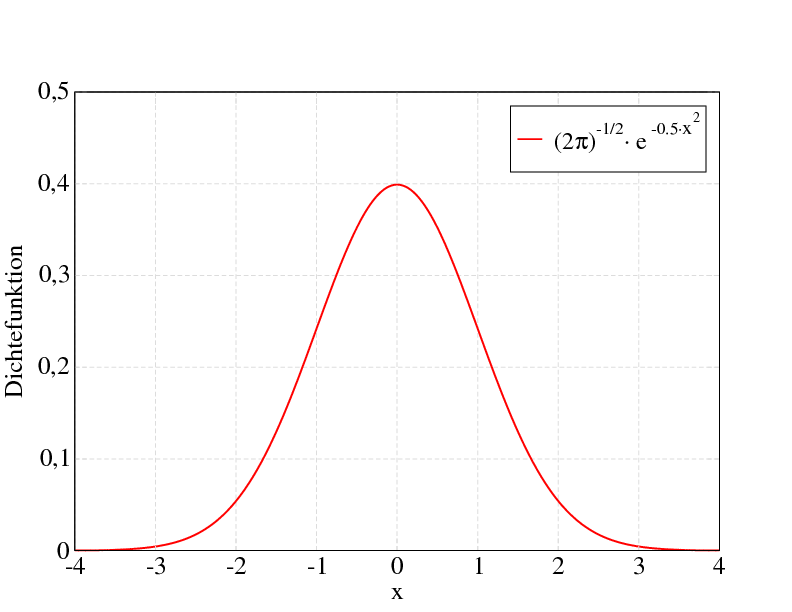
\includegraphics[scale=0.25]{Dichtefunktion_StNorm.png}\\
	Das \footnote{Quelle \href{http://de.wikipedia.org/wiki/Normalverteilung}{Wikipedia}} ist die so genannte Standard-Normal-Verteilung, auch bekannt als Gau\ss\ 'sche Glockenkurve
	\item 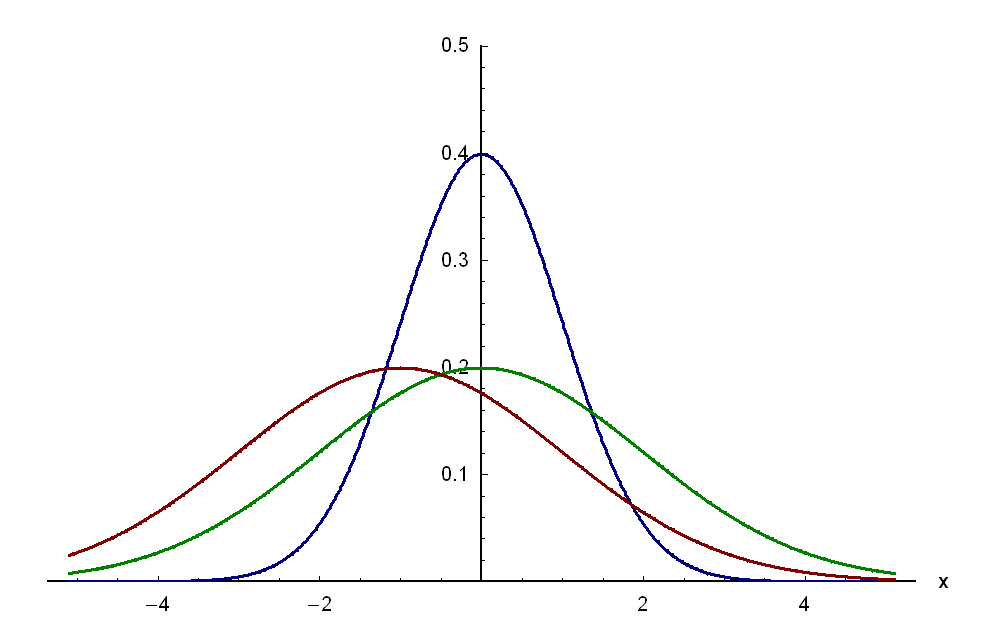
\includegraphics[scale=0.25]{Dichtefunktion_Norms.png}\\
	Zum Vergleich Dichtefunktionen der Normalverteilungen $N(0,1)$ (blau), $N(0,2)$ (gr�n) und $N(-1,2)$ (rot)
\end{itemize}

\subsection{Die Exponential-Verteilung}

\begin{equation}
	f(t) = \begin{cases}
		0 			&,\ t < 0\\
		\lambda \cdot exp(-\lambda t) &,\ t \geq 0
	\end{cases}
\end{equation}

Hierbei sei $\lambda > 0$.

Dann
\begin{equation}
	F(x) = P(X \leq x) = \begin{cases}
		0 			&,\ x < 0\\
		1 - exp(-\lambda t) &,\ x \geq 0
	\end{cases}
\end{equation}

$X$ hei�t Exponential-verteilt mit dem Parameter $\lambda > 0$.
Schreibweise:
\begin{equation}
	X \sim Exp(\lambda)
\end{equation}

% neuer abschnitt?

$X:\Omega \rightarrow \mathbb{R}^2$ sei ein 2-dimensoinaler Zufalsvektor, $X=(X_1,X_2)$.
$X$ habe die Dichte $f(\geq 0)$, d.h.
\begin{equation}
	\begin{split}
		P(X_1 \leq x_1, X_2 \leq x_2) &= \int_{-\infty}^{x_2}{\left( \int_{-\infty}^{x_1}{f(t_1,t_2) dt_2} \right)dt_1} \\
																	&= \int_{-\infty}^{x_1}{\left( \int_{-\infty}^{x_2}{f(t_1,t_2) dt_1} \right)dt_2}
	\end{split}
\end{equation}

Dann ist
\begin{equation}
	\begin{split}
		P(X_1 \leq x_1) &= \int_{-\infty}^{x_1}{\left( \int_{-\infty}^{+ \infty}{f(t_1,t_2) dt_2} \right)dt_1} \\
										&= \int_{- \infty}^{x_1}{f_{X_1}(t_1) dt_1}
	\end{split}
\end{equation}

Also ist 
\begin{equation}
	f_{X_1}(t_1) = \int_{- \infty}^{+ \infty}{f(t_1,t_2)dt_2},\ -\infty < t_1 < + \infty
\end{equation}
Dichte von $X_1$

Analog errechnet sich die Dichte von $X_2$

\part{Bedingte Wahrscheinlichkeiten}

\section{Bedingte Wahrscheinlichkeiten}

$(\Omega,\mathfrak{A},P)$ ist W-Raum.
Zun�chst $|\Omega| < \infty,\ \mathfrak{A} = \mathfrak{P}(\Omega),\ P(A)=\frac{|A|}{|\Omega|},\ A \subset \Omega,\ A\subset \Omega, B\subset\Omega, |B| \geq 1$.
Dann
\begin{equation}
	\frac{|A \cap B|}{|B|} = \frac{\frac{|A \cap B|}{|\Omega|}}{\frac{|B|}{|\Omega|}} = \frac{P(A \cap B)}{P(B)}
\end{equation}
"`Wahrscheinlichkeit f�r das Eintreten von A unter Bedingung, dass B eintritt"', lese als "`Wahrscheinlichket von A unter B"'

\subsection{Definition}

$(\Omega,\mathfrak{A},P)$ W-Raum (bel), $A,b \in \mathfrak{A}, P(B)>0$. Dann hei�t
\begin{equation}
	P(A|B) = \frac{P(A \cap B)}{P(B)}
\end{equation}
die bedingte Wahrscheinlichkeit von A unter B ("`A gegeben B"').

\subsection{Satz}

$(\Omega,\mathfrak{A},P)$ W-Raum, $\emptyset \neq I$ abz�hlbare Indexmenge.
Wir unterstellen $A_i \in \mathfrak{A}, i \in I$ seien paarweise disjunkt, $P(A_i) > 0$ f�r jede $i \in I$.
Dann halten wir fest
\begin{enumerate}
	\item F�r $A \in \mathfrak{A}$ mit der Eigenschaft $A \in \sum_{i \in I}{A_1}$ ist $P(A) = \sum_{i \in I}{P(A|A_i)P(A_i)}$ (bekannt als "`Satz von der totalen Wahrscheinlichkeit"')
	\item Sei $A \in \mathfrak{A}$ mit $P(A) > 0, i_0 \in I$. Dann
	\begin{equation}
		P(A_{i_0}|A) = \frac{P(A|A_{i_0})P(A_{i_0})}{\sum_{i \in I}{P(A|A_i)P(A_i)}}
	\end{equation}
	(bekannt als "`Formel von Bayes"')
	\item Sei $I = \{ 0,1,\ldots,n \},\ (n \in \mathbb{N} \text{fest})$. Dann gilt
	\begin{equation}
		P(A_0 \cap A_1 \cap \ldots \cap A_n) = P(A_0)P(A_1|A_0)P(A_2|A_0\cap A_1)\cdots P(A_n|A_0\cap \ldots \cap A_{n-1})
	\end{equation}
	(bekannt als "`Multiplikationsformel"')
\end{enumerate}

\subsection{Beweis}
\begin{enumerate}
	\item Aus \[A = \sum_{i\in I}{(A \cap A_i)} \] folge sofort
	\[ P(A) \sum_{i\in I}{P(A \cap A_i)} = \sum_{i\in I}{P(A|A_i)P(A_i)} \]
	\item folgt sofort aus 1.
	\item \begin{equation}
		\begin{split}
		& P(A_0)P(A_1|A_0)P(A_2|A_0\cap A_1)\cdots P(A_n|A_0\cap \ldots \cap A_{n-1}) \\
		=	& \cancel{P(A_0)}\cdot \frac{\cancel{P(A_1\cap A_0)}}{\cancel{P(A_0)}} \cdot \frac{P(A_0 \cap A_1 \cap A_2)}{\cancel{P(A_0 \cap A_1)}} \cdots \\
		= & P(A_0\cap A_1 \cap \ldots \cap A_n)
		\end{split}
  \end{equation}
\end{enumerate}

\subsection{Beispiel: Lostrommel}

Eine Lostrommel enth�lt $a$ Gewinnlose und $b$ Nieten, $A \geq 1, b \geq 2$. Es gibt $2$ Spielm�glichkeiten:
\begin{enumerate}
	\item Ein Los wird gezogen. Das gezogene Los ist ein Gewinnlos oder eine Niete. Das Spiel ist beendet.
	\item Ein Los wird gezogen und unbesehen weggeworfen. Daraufhin entfernt der Losverk�ufer eine Niete aus der Trommel. Ein weiteres Los wird gezogen. Dieses Los ist ein Gewinnlos oder eine Niete.
\end{enumerate}

Sei $A$ das Ereignis, dass bei der ersten Ziehung ein Gewinnlos gezogen wird.\\
Sei $B$ das Ereignis, dass bei der zweiten Ziehung ein Gewinnlos gezogen wird.

Dann ergibt sich bei diesen F�llen
\begin{enumerate}
	\item \begin{equation}
		P(A) = \frac{a}{a+b}
	\end{equation}
	\item \begin{equation}\begin{split}
		P(B) 	&= P(B|A)\cdot P(A) + P(B|A^c)P(A^c) \\
					&= \frac{a-1}{a+b-2}\cdot \frac{a}{a+b} + \frac{a}{a+b-2} \cdot \frac{b}{a+b} \\
					&= \frac{a}{a+b}\cdot\left(\underbrace{\frac{a+b-1}{a+b-2}}_{\geq 1} \right) > \frac{a}{a+b} > P(A)
		\end{split}
	\end{equation}
	Sei nun $a=1,\ b=2$. Dann folgt sofort
	\begin{equation*}
		\begin{split}
			P(A) &= \frac{1}{3}\\
			P(B) &= \frac{1}{3}\cdot 2 = \frac{2}{3}
		\end{split}
	\end{equation*}
\end{enumerate}

Sei $A,B \in \mathfrak{A}, P(B)>0$. Dann gilt offenbar
\begin{equation}
	P(A|B) = P(A) \iff P(A\cap B) = P(A)P(B)
\end{equation}

\section{Stochastische Unabh�ngigkeit von Ereignissen und Zufallsvariablen}

\subsection{Definition}

$(\Omega,\mathfrak{A},P)$ W-Raum, $A,B \in \mathfrak{A}$. $A,B$ hei�en (stochastisch) unabh�ngig, wenn \[ P(A \cap B) = P(A)P(B) \] gilt.

\subsection{Einsicht / Beweis}

\begin{equation}
	\begin{split}
		P(A \cap B^c)	&= P(A)-P(A \cap B) \\
									&= P(A) - P(A)P(B),\ \text{falls $A,B$ unabh�ngig} \\ % \Rightarrow A,B^c unabh�ngig
									& (1-P(B))P(A) \\
									&= P(A)P(B^c)
	\end{split}
\end{equation}

\subsection{Definition}
\begin{itemize}
	\item $\emptyset \neq I$ endliche Indexmenge, $A_i \in \mathfrak{A}, i \in I$ Ereignisse.\\
				$A_i$ hei�en (stochastisch) unabh�ngig, wenn f�r jede $\emptyset \neq J \subset I$ gilt
				\begin{equation}
					P\left( \bigcap_{j\in J}{A_j} \right) = \prod_{j \in J}{P(A_j)}
				\end{equation}
	\item $\emptyset \neq I$ beliebige Indexmenge, $A_i \in \mathfrak{A}, i \in I$ Ereignisse.\\
				$\mathfrak{A}_i, i \in I$ hei�en unabh�ngig, wenn f�r jede Teilmenge $\emptyset \neq J \subset I,\ J \text{endlich}$ die Ereignisse $A_j,j\in J$ unabh�ngig sind.
\end{itemize}

\subsubsection{Bemerkung}

$A_i \in \mathfrak{A}, i \in I$ seien Ereignisse. Dann gilt
\begin{equation}
	A_i, i\in I \text{ unabh�ngig } \iff B_i, i\in I \text{ unabh�ngig },\ B_i \in \{A_i, A_i^c\} \text{ beliebig}
\end{equation}

\subsection{Definition}

$(\Omega,\mathfrak{A},P)$ W-Raum, $\emptyset \neq I$ Indexmenge, $(R_i,\mathfrak{S})$ Messr�ume, $i \in I$,
$X_i:\Omega \rightarrow R_i$ Zufallsvariable, $i \in I$.\\
$X_i, i\in I$ hei�en (stochastisch) unabh�ngig, wenn f�r jede Wahl von $B_i \in \mathfrak{S}_i, i\in I$ die Ereignisse 
$A_i = X_i^{-1}(B_i), i \in I$ unabh�ngig sind.

%\subsection{Spezialfall}
%$I = \{1,\ldots,n\}$.
%
%$X_i, i \in I$ sind unabh�ngig $\iff P(X_1 \in B_1, \ldots, X_n\in B_n) = P(X_1 \in B_1) \cdots P(X_n\in B_n), \forall B_i \in \mathfrak{S}_i, i \in I$
%
%\begin{enumerate}
%	\item $X_1,\ldots,X_n$ haben eine \textbf{diskrete Verteilung}. Dann
%				\[ X_1,\ldots,X_n \iff P(X_1=x,\ldots,X_n=x_n) = P(X_1=x_1)\cdots P(X_n=x_n)\]
%				f�r jede $x_i \in R_i, i \in I$
%\end{enumerate}


$(\Omega,\mathfrak{A},P)$ sei W-Raum. Dann $X_i:\Omega \Rightarrow R_i,\ i=1,\ldots,n \text{Zufallsvariable}$
$X_1,\ldots,X_n$ sind unabh�ngig, wenn gilt
\[ P(X_1\in B_1,\ldots,X_n\in B_n) = P(X_1\in B_1)\cdots P(X_n\in B_n) \]
f�r jede Auswahl von Ereignissen $B_i \in \mathfrak{A}, i=1,\ldots,n$

\ldots

\subsection{Spezialf�lle}

\subsubsection{Diskrete Verteilung}

Die $X_1,\ldots,X_n$ haben je eine diskrete Verteilung.
			  Dann sind 
			  \[ X_1,\ldots,X_n \text{ unabh�ngig } \iff P(X_1=x_1,\ldots,X_n=x_n) = P(X_1=x_1)\cdots P(X_n = x_n)\] 
			  f�r jede Auswahl von Elementen $x_i \in R_i,\ i=1,\ldots,n$.\\
			  (Beachte hier: $\{x\}\in R_i,\ \forall x\in R,\ \forall i\in I$)

\subsubsection{Stetige Verteilung}

Sei $X=(X_1,\ldots,X_n)$ mit den reellen Zufallsvariablen $X_1,\ldots,X_n$.
				Es habe $X$ eine Dichte $f$, das hei�t
				\[ P(X_1 \leq x_1, \ldots, X_n \leq x_n) = \int_{-\infty}^{x_n} \cdots \int_{-\infty}^{x_1}{f(t_1,\ldots,t_n)dt_1,\ldots,dt_n},\ (x_1,\ldots,x_n \in R^n) \]
				Dann hat $X_i$ die Dichte
				\[ f_i(x_i) = \int_{-\infty}^{+\infty} \cdots 	\int_{-\infty}^{+\infty}{f(t_1,\ldots,t_{i-1},x_i,t_{i+1},\ldots,t_n)dt_1,\ldots,dt_n} \]

Gilt
\begin{equation}
	f(x_1,\ldots,x_n) = \prod_{i=1}^{n}{f_i(x_i)},\ (x_1,\ldots,x_n)\in\mathbb{R}^n
\end{equation}
so sind die Zufallsvariablen $X_1,\ldots,X_n$ unabh�ngig.

\subsection{Beispiel}
Ein Einzelexperiment, bei dem ein interessierendes Ereignis $A$ mit Wahrscheinlichkeit $p\in [0,1]$ eintritt, wird $n$-mal unter identischen Versuchsbedingungen ohne gegenseitige Beeinflussung (unabh�ngige Versuchswiederholungen) wiederholt.\\
Beschreibe das Einzelexperiment durch den W-Raum $(\Omega_0,\mathfrak{A}_0,P_0)=(\{0,1\}, \mathfrak{P}(\{0,1\}),P_0)$ mit 
\begin{itemize}
	\item $P_0(\{0\})=1-p$
	\item $P_0(\{1\})=p$
	\item $0 \cong A \text{ tritt nicht ein}$
	\item $1 \cong A \text{ tritt ein}$
\end{itemize}

Beschreibe das Gesamtexperiment durch
\[ (\Omega,\mathfrak{A},P) \text{ mit } \Omega=\{0,1\}^n=\{(\omega_1,\ldots,\omega_n); \omega_i \in \{0,1\}, i=1,\ldots,n\}, \mathfrak{A}=\mathfrak{P}(\Omega) \]
\begin{equation}
	\begin{split}
		P(\{\omega_1,\ldots,\omega_n\}) &= P_0(\{\omega_1\})\cdot P_0(\{\omega_n\}) \\
																		&= p^{\omega_1}\cdot (1-p)^{1-\omega_1}\cdots p^{w_n}\cdot(1-p)^{1-\omega_n} \\
																		&= p^{\omega_1+\ldots+\omega_n}\cdot (1-p)^{n-(\omega_1+\ldots+\omega_n)}, (\omega_1,\ldots,\omega_n) \in \Omega
	\end{split}
\end{equation}

$X_i:\Omega\rightarrow\{0,1\}$ sei definiert durch
\[ X_i(\omega_1,\ldots,\omega_n) = \omega_i, (\omega_1,\ldots,\omega_n)\in\Omega, i=1,\ldots,n \]
Die $X_1,\ldots,X_n$ sind unabh�ngig, denn
\begin{equation}
	\begin{split}
		&P(X_1=\epsilon_1,\ldots,X_n=\epsilon_n) \\
	= &P(\text{w1toninOmega};\ X_1(\omega_1,\ldots,\omega_n)=\epsilon_1,\ldots,X_n(\omega_1,\ldots,\omega_n)=\epsilon_n) \\
	=	& P(\{(\epsilon_1,\ldots,\epsilon_n)\}\\
	=	& p^{\epsilon_1+\ldots+\epsilon_n}\cdot(1-p)^{n-(\epsilon_1+\ldots+\epsilon_n)} \\
	=	& \prod_{i=1}^{n}{p_i^{\epsilon_i}\cdot(1-p)^{1-\epsilon_i}}
	\end{split}
\end{equation}

\begin{equation}
	\begin{split}
		P(X_1=\epsilon_1) &= P(\{(\omega_1,\ldots,\omega_n)\in\Omega; X_1(\omega_1,\ldots,\omega_n)=\epsilon_1\}) \\
											&= P(\{ (\epsilon_1,\omega_2,\ldots,\omega_n); \omega_i\in\{0,1\}, 2\leq i\leq n \}) \\
											&= \sum_{nnn}{P}\ldots
	\end{split}
\end{equation}

\begin{equation}
	\begin{split}
		P(X=k) &= \ldots
	\end{split}
\end{equation}

\section{Definition: Binomialverteilung}

Eine reelle (oder $\{0,1\}$-wertige) Zufallsvariable $X$ hei�t Binomailverteilt mit den Parametern $n\in\mathbb{N}$ und $p\in[0,1]$, wenn gilt
\begin{equation}
	P(X=k) = \binom{n}{k}\cdot p^k \cdot (1-p)^{n-k}, k \in \{0,1,\ldots,n\}
\end{equation}
Schreibweise: \[ X \sim \mathfrak{B}(n,p) \]

\subsection{Anwendung}
Sei $(\Omega,\mathfrak{A},P)$ W-Raum, $A\in \mathfrak{A}$ Ereignis. Dann hei�t $I_A:\Omega \rightarrow \{0,1\}$ \textbf{Indikator} (oder Indikatorvariable) von $A$, definiert durch
\[ I_A(\omega) = \begin{cases}
	1, &\ \omega \in A \\
	0, &\ \omega \notin A.
\end{cases} \]

$I_A \sim \mathfrak{B}(1,p)$ mit $p=P(A)$.\\
Seien $A_1,\ldots,A_n\in \mathfrak{A}$ unabh�ngige Ereignisse mit $p=P(A_i), i=1,\ldots,n.$.\\
Dann gilt $\underbrace{X_1}_{=I_{A_1}},\ldots,\underbrace{X_n}_{=I_{A_n}}$ unabh�ngig und $X_i \sim \mathfrak{B}(1,p)$. $X=X_1+\ldots+X_n \sim \mathfrak{B}(n,p)$.

\subsection{Beispiel Urnenmodell}

Eine Urne enth�lt $r$ rote und $s$ schwarze Kugeln. Uns k�nnen verschiedene Modi interessieren.

\subsubsection{Mit Zur�cklegen}

Es wird $n$-mal mit Zur�cklegen je eine Kugel gezogen.\\
Sei $X$ Zufallsvariable und bezeichne die Anzahl der gezogenen roten Kugeln in $n$ Ziehungen.\\
Dann $X \sim \mathfrak{B}\left(n,\frac{r}{r+s}\right)$

\subsubsection{Ohne Zur�cklegen}

Es wird $n$-mal ohne Zur�cklegen je eine Kugel gezogen mit $n\leq r+s =: a$.\\
				Sei $X$ Zufallsvariable und bezeichne die Anzahl der gezogenen roten Kugeln in $n$ Ziehungen.\\
				Nummeriere die Kugeln in folgender Weise:
				\[\underbrace{1,\ldots,r}_{\text{rot}},\underbrace{r+1,\ldots,\overbrace{r+s}^{=a}}_{\text{schwarz}}\]
				Dann
				\begin{itemize}
					\item $\Omega=\{(\omega_1,\ldots,\omega_n);\ \omega_i\in\{1,\ldots,a\} \text{paarweise verschieden}, 1\leq i \leq n \}$
					\item $\mathfrak{A}=\mathfrak{P}(\Omega)$
					\item $P(A) = \frac{|A|}{|\Omega|}=\frac{|A|}{a\cdot(a-1)\cdot(a-n+1)},\ A\subset\Omega$
					\item \begin{equation}
								\begin{split}
									P(X=k) &= \frac{|\{(\omega_1,\ldots,\omega_n)\in\Omega; |j\in \{1,\ldots,n\}, \omega_j\in\{1,\ldots,r\}|=k\}|}{|\Omega|}\\
												 &= \frac{\binom{n}{k}\cdot r\cdot(r-1)\cdots(r-k+1)\cdot s\cdot(s-1)\cdots(s-(n-k)+1)}{a\cdot(a-1)\cdots(a-n+1)} \\
												 &= \frac{\binom{r}{k}\cdot\binom{a-r}{n-k}}{\binom{a}{n}}, k\in\mathbb{N}, max(0,a-r-n)\leq k \leq min(n,r)
								\end{split}
								\end{equation}
				\end{itemize}

\section{Definition: Hypergeometrische Verteilung}

Eine reelle Zufallsvariable mit der Verteilung
\[ P(X=k) = \frac{\binom{r}{k}\cdot\binom{a-r}{n-k}}{\binom{a}{n}} \]
hei�t hypergeometrisch verteilt mit den Parametern $a,r,n\in\mathbb{N}, r\leq a, n\leq a$ und der Schreibweise
\begin{equation}
	X \sim \mathfrak{H}(a,r,n).
\end{equation}

Das bekannteste Beispiel d�rfte das Zahlenlotto ``6 aus 49'' sein.

\end{document}